% ---------------------------------------------------------------------------- %
\section{Linguometer Results}
\label{ch:results}
% ---------------------------------------------------------------------------- %
In this Section, the results obtained
thus far with the Linguometer are presented.
The main result accomplished
is the simultaneous acquisition of phono-articulatory features and the
consequent alignment via the \emph{LMTools2} toolkit.
It is important to clarify that out of the nine recorded experiments, three 
have been dropped due to recording problems.
Specifically, the audio mixer (\wf{AMX}) broke down during the second
experiment, failing to generate the segmentation signals with the main speech 
signal acquired via \wf{MIC0}.
Furthermore, during the third experiment the articulograph software kept 
crashing, and it had been necessary to reboot the control computer various
times.
% ---------------------------------------------------------------------------- %
\begin{figure}[htbp]
	\centering
	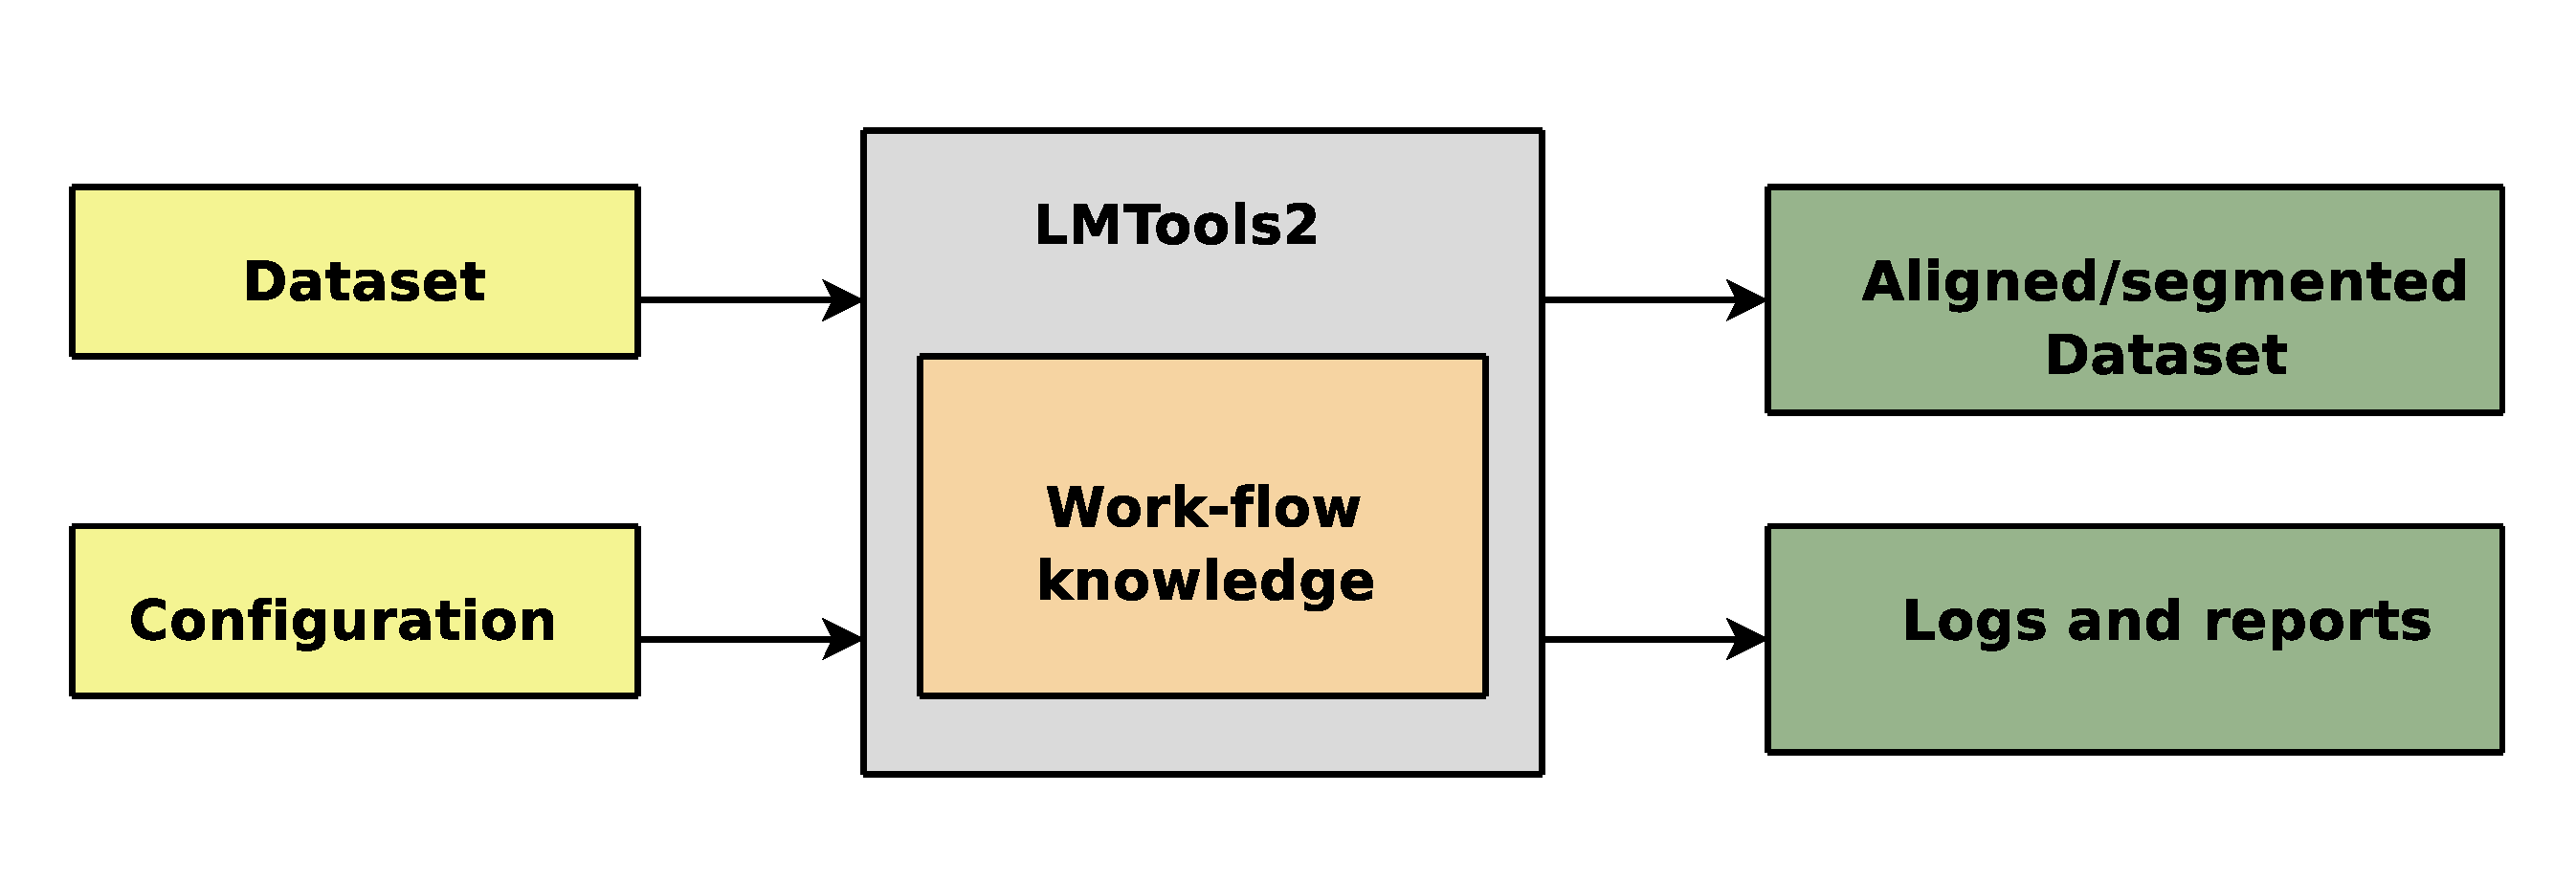
\epsfig{file=include/results/images/blackbox.eps, width=0.75\textwidth}
	\caption[LMTools2 diagram]{\textbf{LMTools2 diagram}: the \emph{LMTools2}
	toolkit operates on the dataset performing alignment and segmentation
	operations. It requires the user to compile a total of three configuration
	files, the rest of the processing is performed without the need of user
	interaction. The toolkit has been integrated using the knowledge of the
	workflow diagram, but adding new features is possible.
	The method proposed by the author produces a packaged version of the
	dataset and many informative logs and plots.}
	\label{fig:results:blackbox}
\end{figure}
% ---------------------------------------------------------------------------- %

Although those two experiments have not been recorded properly, the acquired 
data is not totally unusable.
On the other hand, the seventh experiment has been dropped since the recorded 
male subject moved extensively during the whole acquisition, often complaining
about throat pain and increased salivation.
Under those conditions the subject gets easily stressed out, performing
large head and torso movements.
As a consequence of torso movements, the articulograph frame of reference may
move, thus altering the relative position of the ultrasonographic transducer.

%As far as the author is concerned, the Linguometer integration has to be 
%considered as a result by itself, and for this reason separating the
%implementation from the results turns out to be a tangled task.
%Moreover
%the Linguometer is a personal solution provided by the author for the
%problem of acquiring simultaneously a vast set of phono-articulatory
%parameters.

% ---------------------------------------------------------------------------- %
%\section{Alignment and segmentation}
%\label{sec:results:alignment}
% ---------------------------------------------------------------------------- %
\subsection{Initial alignment and segmentation}
%A total of nine subjects have been recorded using the Linguometer setup,
%following the experimental protocol described in Section~\ref{ch:experiments}.
%In Section~\ref{ch:linguometer:architecture} the workflow and the data-stream
%diagrams have been presented in detail.
%The goal of this Section is to present the methods that allowed the author to
%align and segment the acquired dataset.
%
%It is important to underline that the data is acquired simultaneously, but the
%real synchronization happens in post-processing, using a collection of tools
% called \emph{LMTools2}.
%However \emph{LMTools1} and \emph{LMTools2} share the same name, they were coded
%with completely different tasks in mind.
%In fact, \emph{LMTools} is used to control the whole Linguometer setup, spanning
%from stimuli presentation to data-acquisition and storing.
%On the other hand, \emph{LMTools2} was written to automatically process large
%sets of data acquired using the well determined procedure described in the
%workflow diagram.
%
%It has been said many times that the Linguometer is a constellation of hardware
%and software used to acquire phono-articulatory features, and probably no better
%definition exists.
%The goal met by the Linguometer is the fact that a large dataset of features has
%been acquired and successfully aligned.
%The novel idea behind the Linguometer 
%In fact, the Linguometer setup has been integrated to meet three specifics.
%Firstly, the setup has been developed to be ergonomic, since speech production
%could easily be impaired if the recorded subjects distract themselves.
%Furthermore, the workflow needs to be stable and flexible, in order to recover
%easily from the problems that affect a small set of devices.
%Lastly, the data recorded by the means of the workflow diagram does need to 
%allow to batch-process the recorded data with the smallest possible degree of
%human interaction.
%While the first two topics have been discussed under many aspects in
%Section~\ref{ch:linguometer} and~\ref{ch:experiments}, the latest is described
%in this Section, albeit with some degree of abstraction.\\

The \emph{LMTools2} toolkit is a collection of programs, libraries and
scripts, coded using different languages, such as C/C++, Matlab, Perl and Bash.
The C/C++ programs are used for tasks that require speed and are generally
resource-intensive, such as the detection of the synchronization and the
segmentation peaks. 
Those programs rely on a small set of optimized objects that provide an
abstract interface to data-streams and to the decoding/encoding operations.
Furthermore, particular objects are used to perform peak-detection, signal
segmentation and alignment and similar operations.
Although those programs have some level of adaptive behavior that allow them
to recover, and eventually fix, odd behaviors, the user can easily perform
some tuning writing his own configuration files.

Generally speaking Matlab libraries and scripts are used to perform
data-analysis, plotting results and similar tasks.
Moreover, Matlab is used also to filter and align signals with an
high degree of precision.

C/C++ programs and Matlab scripts provide a consistent and uniform interface to
the data-set.
The task of launching the atomic-level programs is handled by a set of
\emph{LMTools2} scripts mainly written in Perl.
Under normal conditions, a couple of minutes are required to write
experiment-specific configuration files, and almost 5 hours of processing 
are required to align and segment completely a single
experiment.
Figure~\ref{fig:results:blackbox} shows an example \emph{LMTools2} block
diagram.
The alignment procedure can be split into two main stages: a first ``rough''
alignment and a final ``accurate'' alignment.
The need for a rough alignment stage arises from the fact that the dataset
is not recorded with a single time resolution (e.g.: 25~fps video tracks from
\wf{CC} and \wf{AG}, 200~Hz kinesthetic information from articulography data,
16~to 48~kHz audio streams).
In the final stage, where accurate alignment occurs, the data is resampled,
filtered and finally aligned.
Many technical issues have been solved and many adaptive procedures have been
integrated into the \emph{LMTools2} toolkit\footnote{The \emph{LMTools2}
toolkit sources are available and well documented, at: http://yarp0.cvs.sourceforge.net/yarp0/}.
%
%
%
After the alignment has been performed, the signals are cropped so that they 
have the same length in samples. At this point the word-related data is saved to
standard Matlab ``MAT-Files'' and to custom ASCII files, thus allowing the 
processed dataset to be easily shared between the CONTACT Project partners and
in future, to the whole research community.
% ---------------------------------------------------------------------------- %
\subsection{An example of the collected data}
% ---------------------------------------------------------------------------- %
Figures~\ref{fig:results:uovo:aln} and~\ref{fig:results:giallo:aln} show the
diagnostic plots produced by \emph{LMTools2} as a support to the final
validation task.
The two figures illustrate the speech and the EGG signals before and after the
final alignment procedure. As an example, the author choose to use the /uovo/
and the /giallo/ Italian words recorded during the first experiment from a 23
years old female subject (Table~\ref{tab:experiments:subjects}).

% ---------------------------------------------------------------------------- %
\begin{figure}
  \centering
	\subfigure[\label{fig:results:uovo:complex:glasses}]
	{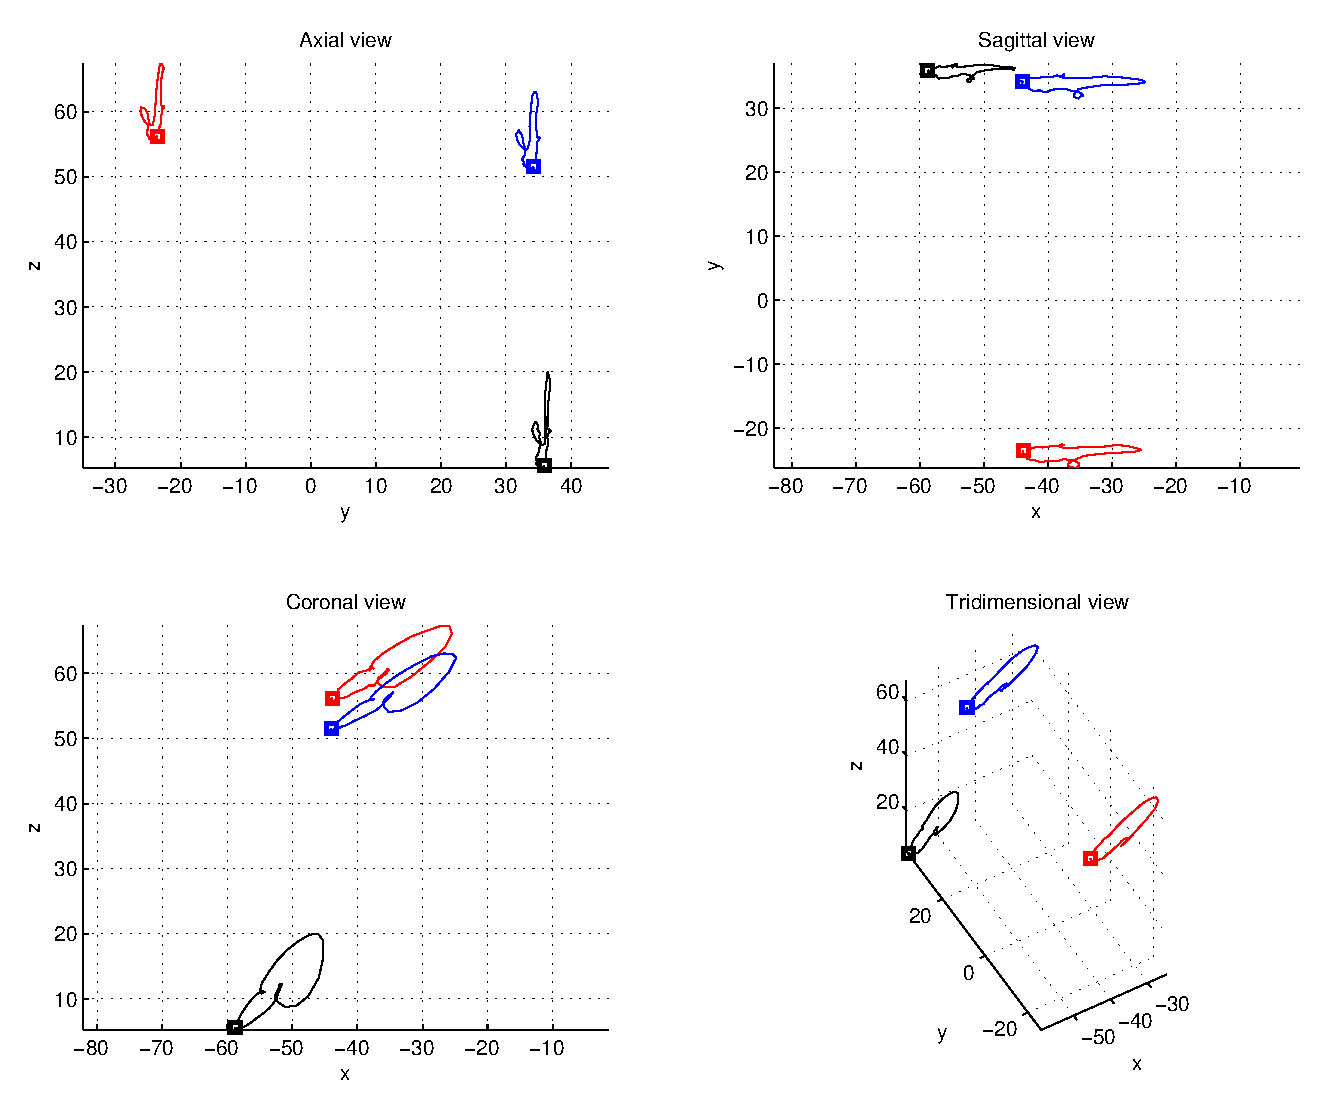
\includegraphics[width=0.45\textwidth]{include/results/images/complex_15_glasses.eps}}
	\hspace{0.05\textwidth}
	\subfigure[\label{fig:results:uovo:complex:tongue}]
	{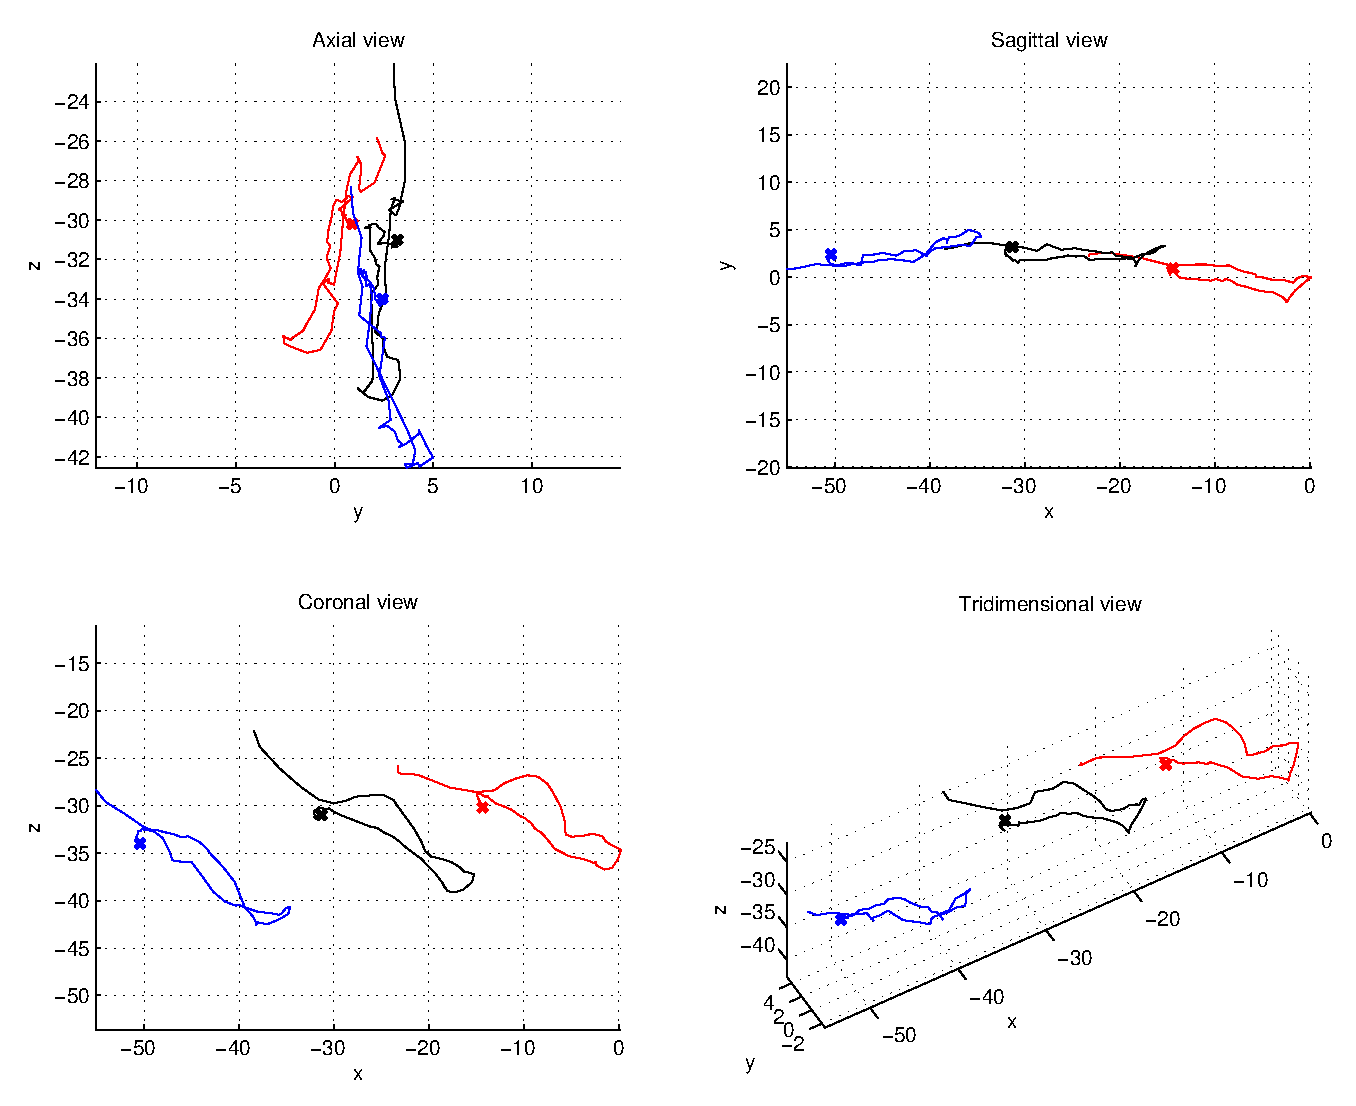
\includegraphics[width=0.45\textwidth]{include/results/images/complex_15_tongue.eps}}

	\caption[Projections of the trajectories of some sensors for 
	/uovo/]{\textbf{Projections of the trajectories of few sensors for /uovo/}: 
	a graphical representation of the trajectories of some sensors is here
	shown for the head-reference sensors (a) and for the three sensors glued 
	sagittally to the dorsum of the tongue (b).
	For each panel (a and b), the axial projection (\emph{yz} plane), 
	the sagittal
	projection (\emph{xy} plane) and the coronal projection (\emph{xz}) are
	shown.
	Furthermore, a tridimensional plot of the trajectories is provided.
	It is important to underline that the subject is looking towards the
	negative direction of the \emph{x} axis.
	Note: (a) sensor 10 in blue, sensor 11 in red and sensor 12 in black; 
	(b) sensor 1 in red, sensor 2 in black and sensor 3 in blue.
	This plot adheres to the convention shown in 
	Figure~\ref{fig:experiments:map}.
	The thick marks indicate the final position of the sensors.
	}
	\label{fig:results:uovo:complex}
\end{figure}
% ---------------------------------------------------------------------------- %

% ---------------------------------------------------------------------------- %
\begin{figure}
  \centering
	\subfigure[\label{fig:results:giallo:complex:glasses}]
	{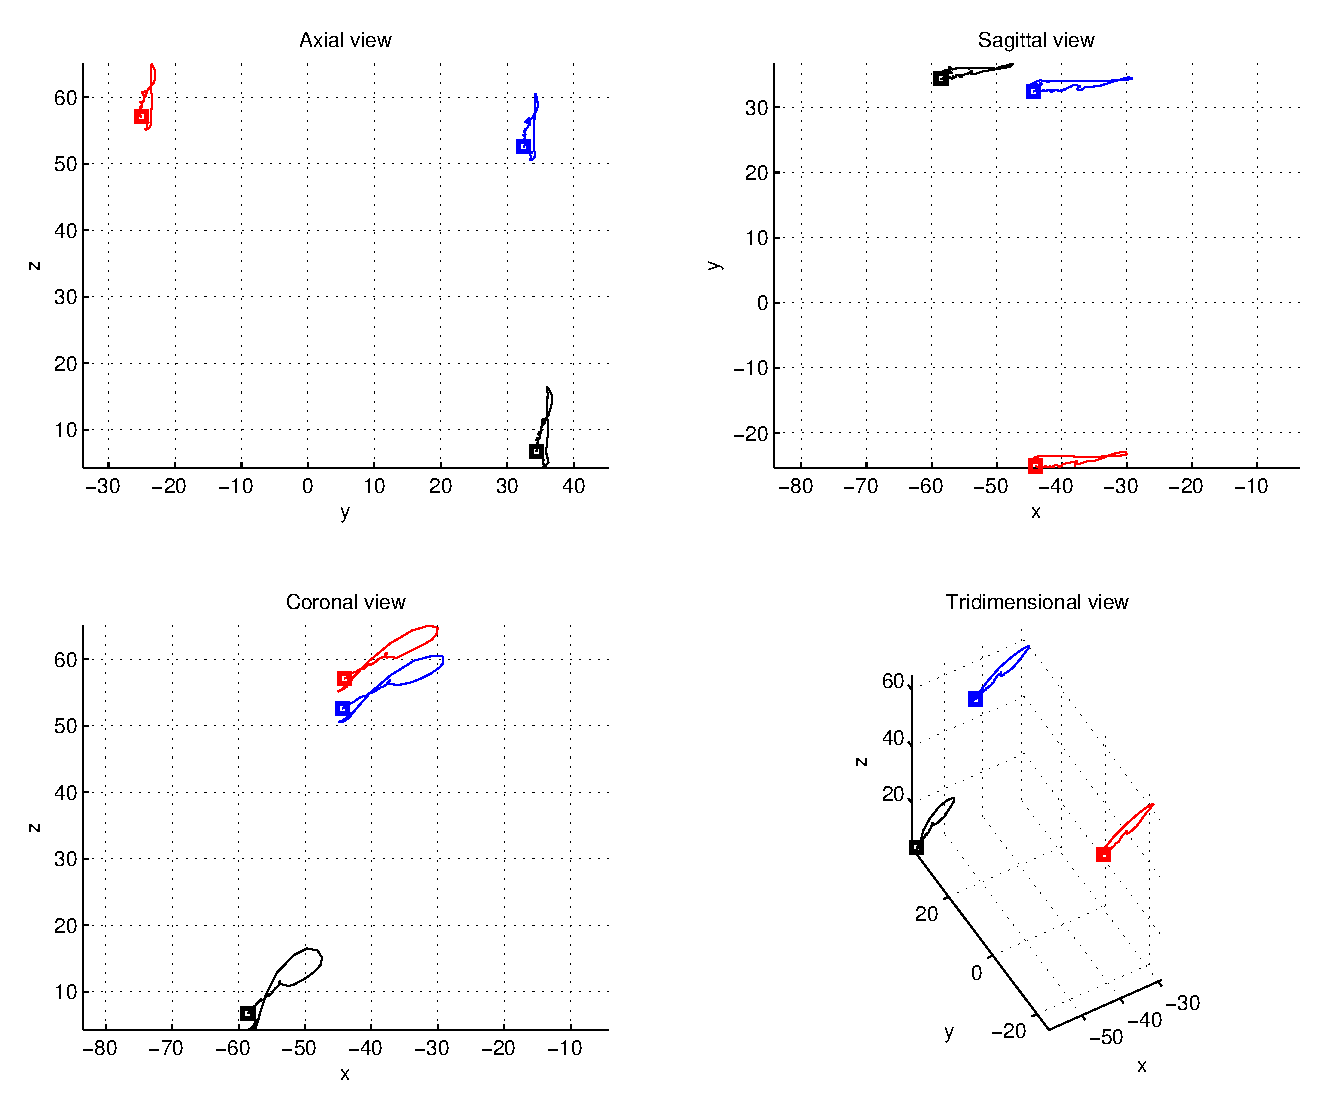
\includegraphics[width=0.45\textwidth]{include/results/images/complex_20_glasses.eps}}
	\hspace{0.05\textwidth}
	\subfigure[\label{fig:results:giallo:complex:tongue}]
	{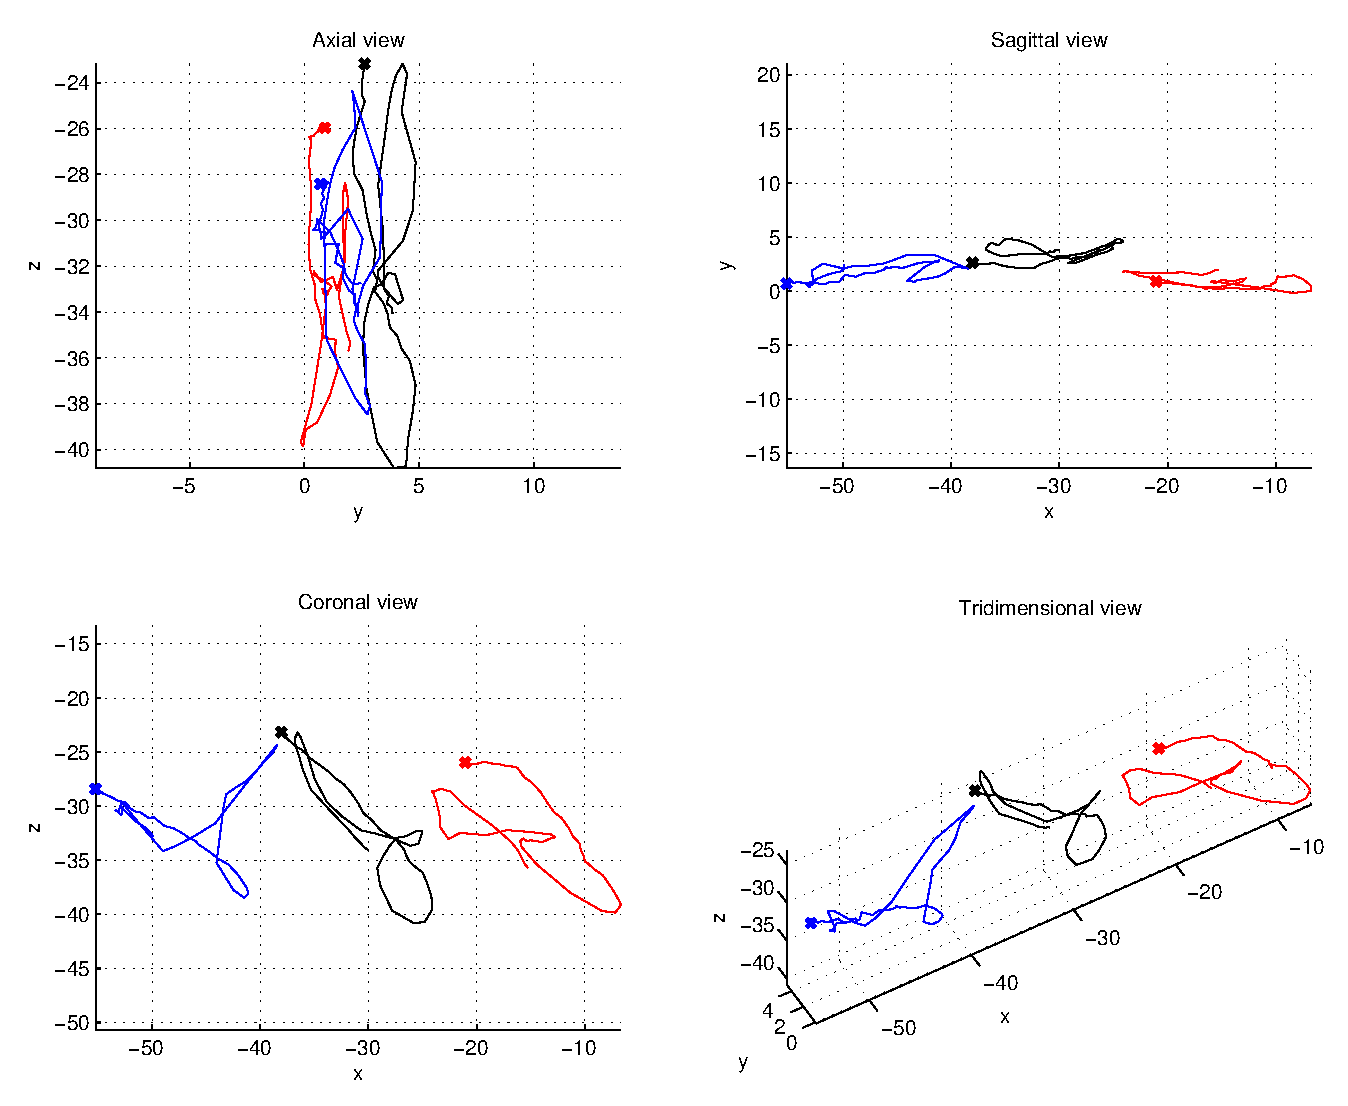
\includegraphics[width=0.45\textwidth]{include/results/images/complex_20_tongue.eps}}

	\caption[Projections of the trajectories of few sensors for /giallo/]{\textbf{Projections of the trajectories of few sensors for /giallo/}: 
	the reader should refer to the caption of
	Figure~\ref{fig:results:uovo:complex}.
	Note: (a) sensor 10 in blue, sensor 11 in red and sensor 12 in black; 
	(b) sensor 1 in red, sensor 2 in black and sensor 3 in blue.
	This plot adheres to the convention shown in 
	Figure~\ref{fig:experiments:map}.
	The thick marks indicate the final position of the sensors.
	}
	\label{fig:results:giallo:complex}
\end{figure}
% ---------------------------------------------------------------------------- %

% ---------------------------------------------------------------------------- %
\begin{figure}
  \centering
	\subfigure[\label{fig:results:mesh:complex:uovo}]
	{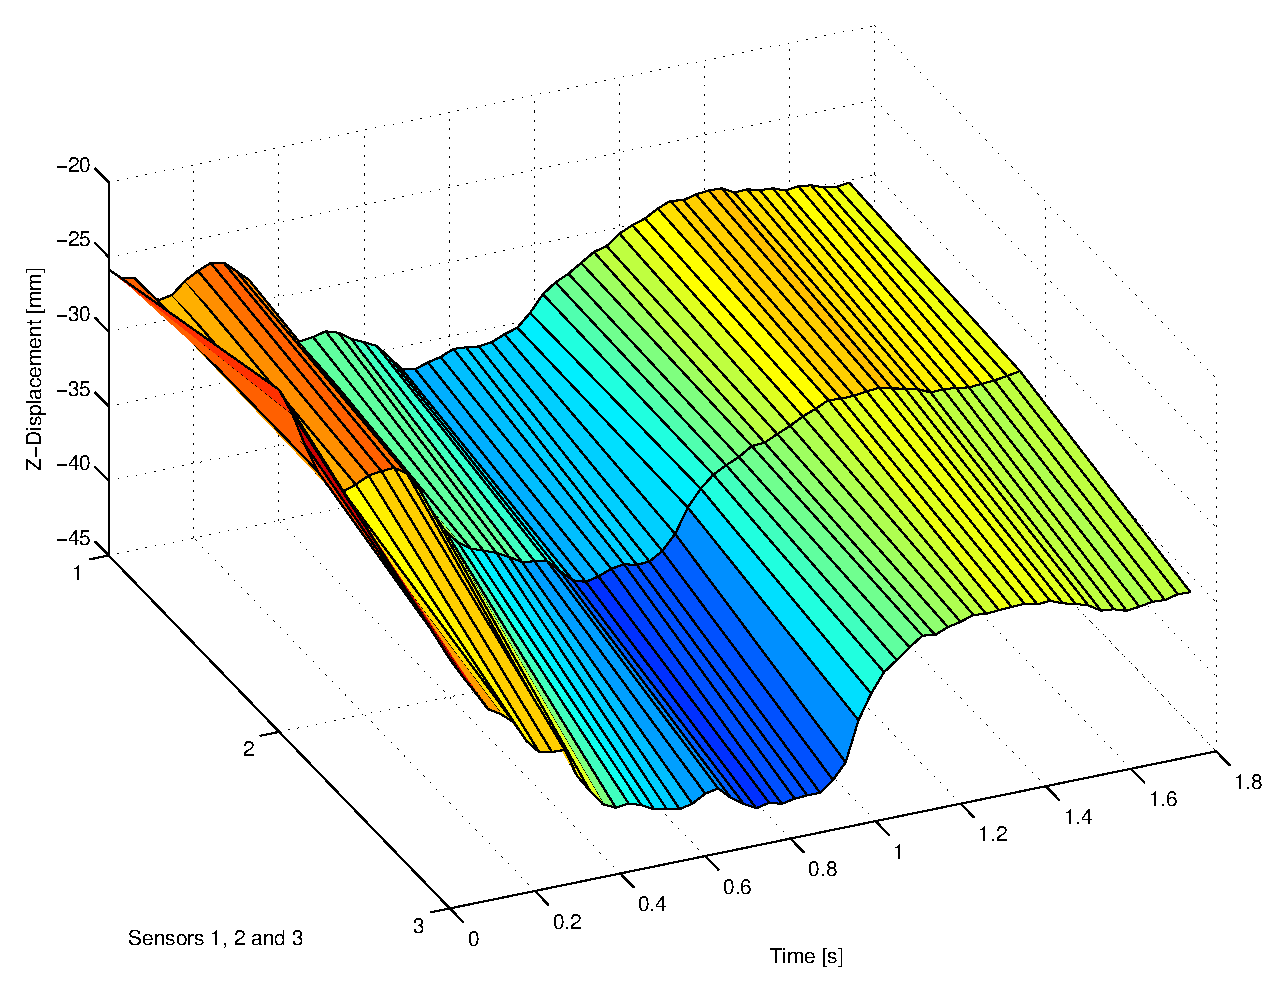
\includegraphics[width=0.45\textwidth]{include/results/images/complex_15_mesh.eps}}
	\hspace{0.05\textwidth}
	\subfigure[\label{fig:results:mesh:complex:giallo}]
	{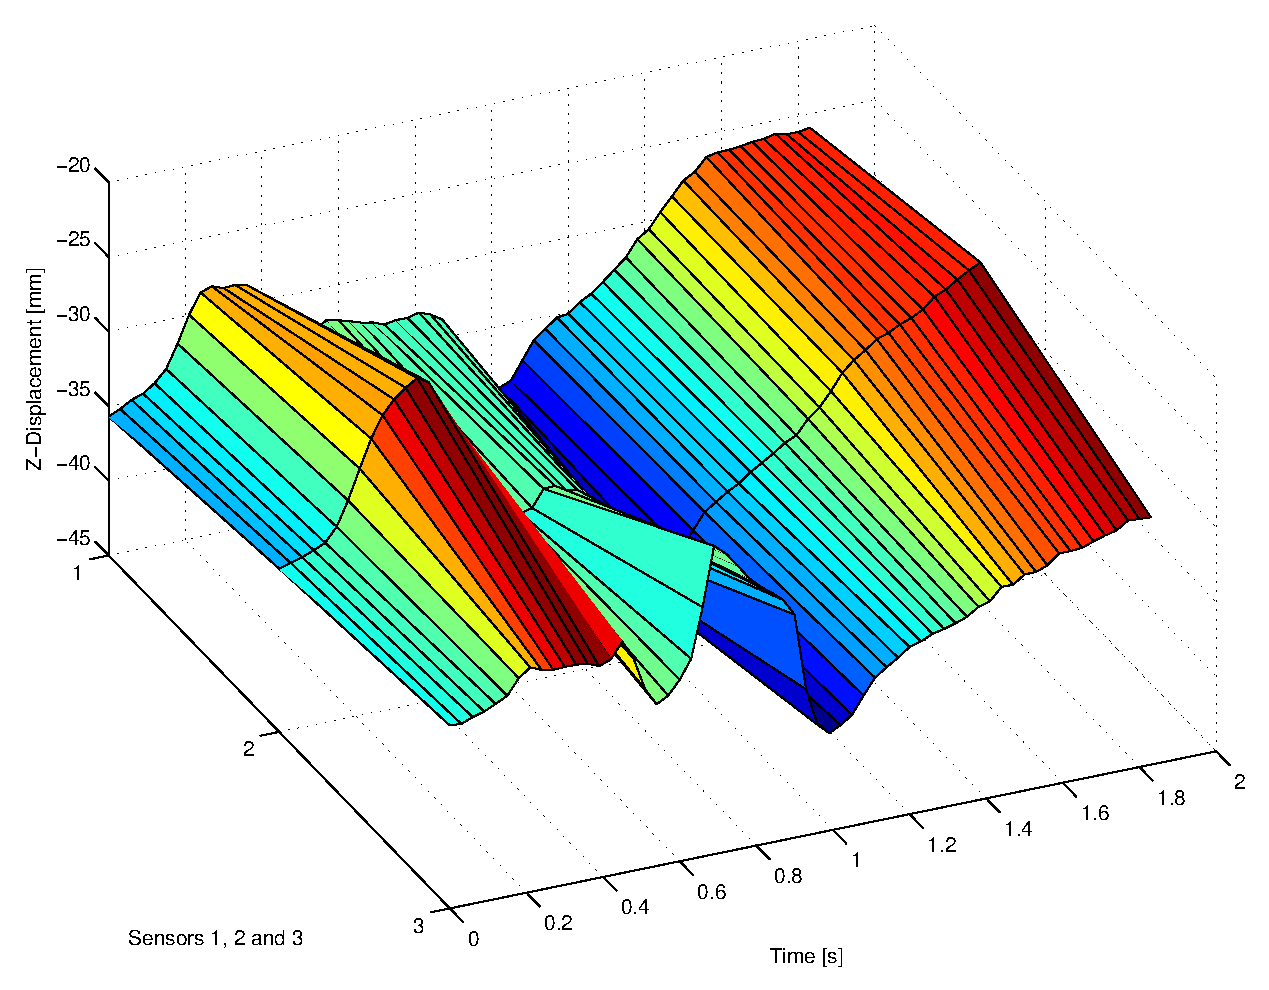
\includegraphics[width=0.45\textwidth]{include/results/images/complex_20_mesh.eps}}

	\caption[Vertical displacement of tongue for /uovo/ and /giallo/ (sagittal
	plane)]{\textbf{Vertical
	displacement of tongue for /uovo/ and /giallo/ (sagittal plane)}: 
	this plot provides a qualitative example for the vertical motion of the
	sensors glued sagittaly onto the tongue dorsum (sensors 1, 2 and 3).
	The kinesthetic information is acquired by the AG500 articulograph at
	a rate of 200 Hz. For the sake of simplicity, the data has been down-sampled
	by a factor of 6 before generating this plot (200 Hz / 6 = 33.3 Hz).
	}
	\label{fig:results:mesh:complex}
\end{figure}
% ---------------------------------------------------------------------------- %

The Cartesian coordinates of trajectories acquired from the twelve sensors 
during the pronunciation of /uovo/ and /giallo/ are shown, from a temporal
perspective, in Figure~\ref{fig:results:trajectories}.
Similarly, Figures~\ref{fig:results:uovo:complex}
and~\ref{fig:results:giallo:complex} show the projections onto the sagittal, 
the axial and the coronal plane of the sensors positioned sagittally onto the 
tongue dorsum and of the sensors taped to the glasses to track head movements.
Those last plots do not include any time information, although the
trajectories of the sensors are fully visible.
By simply looking at the Figures just mentioned, it could be said that the
pronunciation of /uovo/ recruits a more continuous movement of the tongue than
/giallo/. 
It is also clear that during the pronunciation of the submitted stimuli the head
moves, mainly due to jaw motion. 
Moreover, the head reference sensors form, qualitatively, closed-loop
trajectories since the starting point and the ending point overlap. 
Figures~\ref{fig:results:mesh:complex} shows the vertical displacement of the
sensors positioned sagittally onto the tongue dorsum from a spatio-temporal 
perspective.

% ---------------------------------------------------------------------------- %
\begin{figure}
  \centering
	\subfigure[\label{fig:results:ccs:uovo}]
	{\includegraphics[width=0.45\textwidth]{include/results/images/frames_cc_15.tps}}
	\hspace{0.05\textwidth}
	\subfigure[\label{fig:results:ccs:giallo}]
	{\includegraphics[width=0.45\textwidth]{include/results/images/frames_cc_20.tps}}

	\caption[Facial expressions during /uovo/ and /giallo/]{\textbf{Facial 
	expressions during /uovo/ and /giallo/}. 
	Also look at Figures~\ref{fig:results:uovo:cc}
	and~\ref{fig:results:giallo:cc}.}
	
	\label{fig:results:ccs}
\end{figure}
% ---------------------------------------------------------------------------- %

% ---------------------------------------------------------------------------- %
\begin{figure}
  \centering
	\subfigure[\label{fig:results:usss:uovo}]
	{\includegraphics[width=0.45\textwidth]{include/results/images/frames_us_15.tps}}
	\hspace{0.05\textwidth}
	\subfigure[\label{fig:results:uss:giallo}]
	{\includegraphics[width=0.45\textwidth]{include/results/images/frames_us_20.tps}}

	\caption[Tongue motion during /uovo/ and /giallo/]{\textbf{Tongue motion during 
	/uovo/ and /giallo/}: 21 frames extracted from the \wf{US-Video} stream are
	shown. It is important to specify that the images have been cropped.
	Furthermore, in order to enhance the quality of the printed images, a linear
	transformation has been applied so that the colors are inverted.
	Also look at Figures~\ref{fig:results:uovo:us}
	and~\ref{fig:results:giallo:us}.}
	\label{fig:results:uss}
\end{figure}
% ---------------------------------------------------------------------------- %

In order to provide an example of the data acquired using the camcorder and the
ultrasound system, the author used the seeking capabilities of the 
\emph{LMTools2} C++ library combined with the final alignment results.
The onset of speech has been initially detected in the \wf{US-Speech} main 
speech signal recorded during the pronunciation of /uovo/ and /giallo/, using
the finely aligned data packets (the speech signals used for this example are
shown in Figures~\ref{fig:results:uovo:aln} and~\ref{fig:results:giallo:aln}).
Once the onset of speech was detected in the~\wf{US-Speech} signal, that
time instant was marked on the aligned \wf{CC-Speech} signal.
%A similar procedure has been followed to calculate the duration of the speech
%signals.
Once the time instants that characterize the beginning and the end of the
speech signals were known,  the corresponding video
frames were determined for
the \wf{US-Video} and the \wf{CC-Video} streams, thus
extracting  the video frames contained in the previously described interval.
Furthermore, since the seeking operation relies upon the final aligned data,
the extracted frames represent the same physical event, that is the
pronunciation of a word, under different perspectives, such as tongue motion and
facial expressions.
These two specific speech signals happen
to have a very similar time duration: /uovo/
lasts 0.82 seconds, while /giallo/ lasts 0.84 seconds.
since the \wf{US-Video} and the \wf{CC-Video} video streams are acquired at a rate 
of 25 frames per second, the time resolution is 40 milliseconds (e.g.: 1/25Hz =
0.04 seconds).
Since the difference in duration of /uovo/ and /giallo/ is lower than the 
resolution in time of the video streams (e.g.: 0.84 - 0.82 = 0.02), a
total of 21 video frames were extracted from both the steams.

Figure~\ref{fig:results:ccs} shows the 21
video frames extracted from the camcorder stream (\wf{CC-DV}), for both the
pronunciation of /uovo/ and /giallo/.
Similarly, Figure~\ref{fig:results:uss}
shows the 21 frames from the ultrasound system and digitized via the acquisition
card (\wf{ACD}, Section\ref{ch:linguometer:instrumentation:av}).
The representation of those video frames allows the reader to appreciate the
opening and the closing of the mouth, although it is not trivial to perceive
the head movement due to the static nature of the sequence of frames.
It is important to stress the fact that during pronunciation of the submitted
stimuli, the subject moves her head over the sagittal axis, since the
 transducer
stand is rigid. 
In this context, Figure~\ref{fig:results:ccs} is useful to show 
why head compensation plays an important role in the acquisition of the 
kinesthetic information from the sensors attached on the glasses.
% ---------------------------------------------------------------------------- %
% ---------------------------------------------------------------------------- %
\begin{figure}[htbp]
	\centering
	\epsfig{file=include/results/images/frames_cc_15.tps, width=0.75\textwidth}
	\caption[Facial expressions during /uovo/]{\textbf{Facial expressions during /uovo/}.}
	\label{fig:results:uovo:cc}
\end{figure}
% ---------------------------------------------------------------------------- %

% ---------------------------------------------------------------------------- %
\begin{figure}[htbp]
	\centering
	\epsfig{file=include/results/images/frames_cc_20.tps, width=0.75\textwidth}
	\caption[Facial expressions during /giallo/]{\textbf{Facial expressions during /giallo/}
	.}
	\label{fig:results:giallo:cc}
\end{figure}
% ---------------------------------------------------------------------------- %

% ---------------------------------------------------------------------------- %
\begin{figure}[htbp]
	\centering
	\epsfig{file=include/results/images/frames_us_15.tps, width=0.75\textwidth}
	\caption[Tongue profile during /uovo/]{\textbf{Tongue profile during /uovo/}
	.}
	\label{fig:results:uovo:us}
\end{figure}
% ---------------------------------------------------------------------------- %

% ---------------------------------------------------------------------------- %
\begin{figure}[htbp]
	\centering
	\epsfig{file=include/results/images/frames_us_20.tps, width=0.75\textwidth}
	\caption[Tongue profile during /giallo/]{\textbf{Tongue profile during /giallo/}.}
	\label{fig:results:giallo:us}
\end{figure}
% ---------------------------------------------------------------------------- %

\clearpage

